\subsection{Auswertung}
\begin{table}[!h]
	\centering
	\begin{tabular}{|c||c|c|c||c|c|c|}
		\hline
		\multirow{2}{*}{s} & \multicolumn{3}{c||}{Gammaverteilung} & \multicolumn{3}{c|}{Normalverteilung}\\
		\cline{2-7}
		 & \(E\left(F_{end}\right)\) & \(E\left(F_{anf}\right)\) & \(E\left(F\right)\) & \(E\left(F_{end}\right)\) & \(E\left(F_{anf}\right)\) & \(E\left(F\right)\)  \\
		\hline
		73,500 & 5,6650 & 0,0173 & 5,648 & 5,1500 & 0 & 5,150 \\
		73,600 & 5,6384 & 0,0172 & 5,621 & 5,1196 & 0 & 5,120 \\
		73,700 & 5,6118 & 0,0171 & 5,595 & 5,0893 & 0 & 5,089 \\
		73,800 & 5,5854 & 0,0170 & 5,568 & 5,0591 & 0 & 5,059 \\
		73,900 & 5,5590 & 0,0169 & 5,542 & 5,0291 & 0 & 5,029 \\
		73,950 & 5,5459 & 0,0168 & 5,529 & 5,0141 & 0 & 5,014 \\
		73,980 & 5,5380 & 0,0168 & 5,521 & 5,0052 & 0 & 5,005 \\
		\hline
		73,996 & 5,5339 & 0,0168 & 5,517 & 5,0004 & 0 & \cellcolor[gray]{0.8} 5,000 \\
		\hline
		74,020 & 5,5276 & 0,0168 & 5,511 & 4,9932 & 0 & 4,993 \\
		74,050 & 5,5197 & 0,0167 & 5,503 & 4,9843 & 0 & 4,984 \\
		74,080 & 5,5119 & 0,0167 & 5,495 & 4,9754 & 0 & 4,975 \\
		74,100 & 5,5067 & 0,0167 & 5,490 & 4,9694 & 0 & 4,969 \\
		74,200 & 5,4807 & 0,0166 & 5,464 & 4,9398 & 0 & 4,940 \\
		74,300 & 5,4547 & 0,0165 & 5,438 & 4,9103 & 0 & 4,910 \\
		74,400 & 5,4289 & 0,0163 & 5,413 & 4,8809 & 0 & 4,881 \\
		74,500 & 5,4032 & 0,0162 & 5,387 & 4,8516 & 0 & 4,852 \\
		74,600 & 5,3776 & 0,0161 & 5,362 & 4,8225 & 0 & 4,823 \\
		74,700 & 5,3521 & 0,0160 & 5,336 & 4,7935 & 0 & 4,794 \\
		74,800 & 5,3268 & 0,0159 & 5,311 & 4,7647 & 0 & 4,765 \\
		74,900 & 5,3015 & 0,0158 & 5,286 & 4,7359 & 0 & 4,736 \\
		75,000 & 5,2763 & 0,0157 & 5,261 & 4,7073 & 0 & 4,707 \\
		75,100 & 5,2512 & 0,0156 & 5,236 & 4,6789 & 0 & 4,679 \\
		75,200 & 5,2262 & 0,0155 & 5,211 & 4,6505 & 0 & 4,651 \\
		75,300 & 5,2014 & 0,0154 & 5,186 & 4,6223 & 0 & 4,622 \\
		75,400 & 5,1766 & 0,0153 & 5,161 & 4,5942 & 0 & 4,594 \\
		75,500 & 5,1519 & 0,0152 & 5,137 & 4,5663 & 0 & 4,566 \\
		75,600 & 5,1274 & 0,0151 & 5,112 & 4,5384 & 0 & 4,538 \\
		75,700 & 5,1029 & 0,0150 & 5,088 & 4,5107 & 0 & 4,511 \\
		75,800 & 5,0785 & 0,0149 & 5,064 & 4,4831 & 0 & 4,483 \\
		75,900 & 5,0543 & 0,0148 & 5,039 & 4,4557 & 0 & 4,456 \\
		76,020 & 5,0253 & 0,0147 & 5,011 & 4,4229 & 0 & 4,423 \\
		\hline
		76,066 & 5,0142 & 0,0147 & \cellcolor[gray]{0.8} 5,000 & 4,4104 & 0 & 4,410 \\
		\hline
		76,086 & 5,0094 & 0,0146 & 4,995 & 4,4049 & 0 & 4,405 \\
		76,100 & 5,0060 & 0,0146 & 4,991 & 4,4011 & 0 & 4,401 \\
		76,300 & 4,9582 & 0,0144 & 4,944 & 4,3471 & 0 & 4,347 \\
		76,400 & 4,9345 & 0,0143 & 4,920 & 4,3203 & 0 & 4,320 \\
		76,500 & 4,9108 & 0,0142 & 4,897 & 4,2936 & 0 & 4,294 \\
		\hline
	\end{tabular}
	\caption{Ermittlung von $s_{opt}$ über den Erwartungswert der Fehlmenge}
	\label{tab:auswertung}
\end{table}
\pagebreak

Stellt man die Tabelle \ref{tab:auswertung} mit äquidistanten Werten für s in Form eines Diagramms dar, so ergibt sich die Grafik \ref{img:vergleich}. Die Markierungen kennzeichnen die gesuchten Zielwerte für die beiden Verteilungsfunktionen. Die zugehörigen x-Werte der Markierungen entsprechen den Werten für \(s_{opt}\).

Es kann beobachtet werden, dass die Normalverteilung im Vergleich zur Gammaverteilung einen um \(76,1\text{ Stk.}-74,0\text{ Stk.}=2,1\text{ Stk.}\) geringeren optimalen Bestellpunkt besitzt.

\begin{figure}
	\centering
	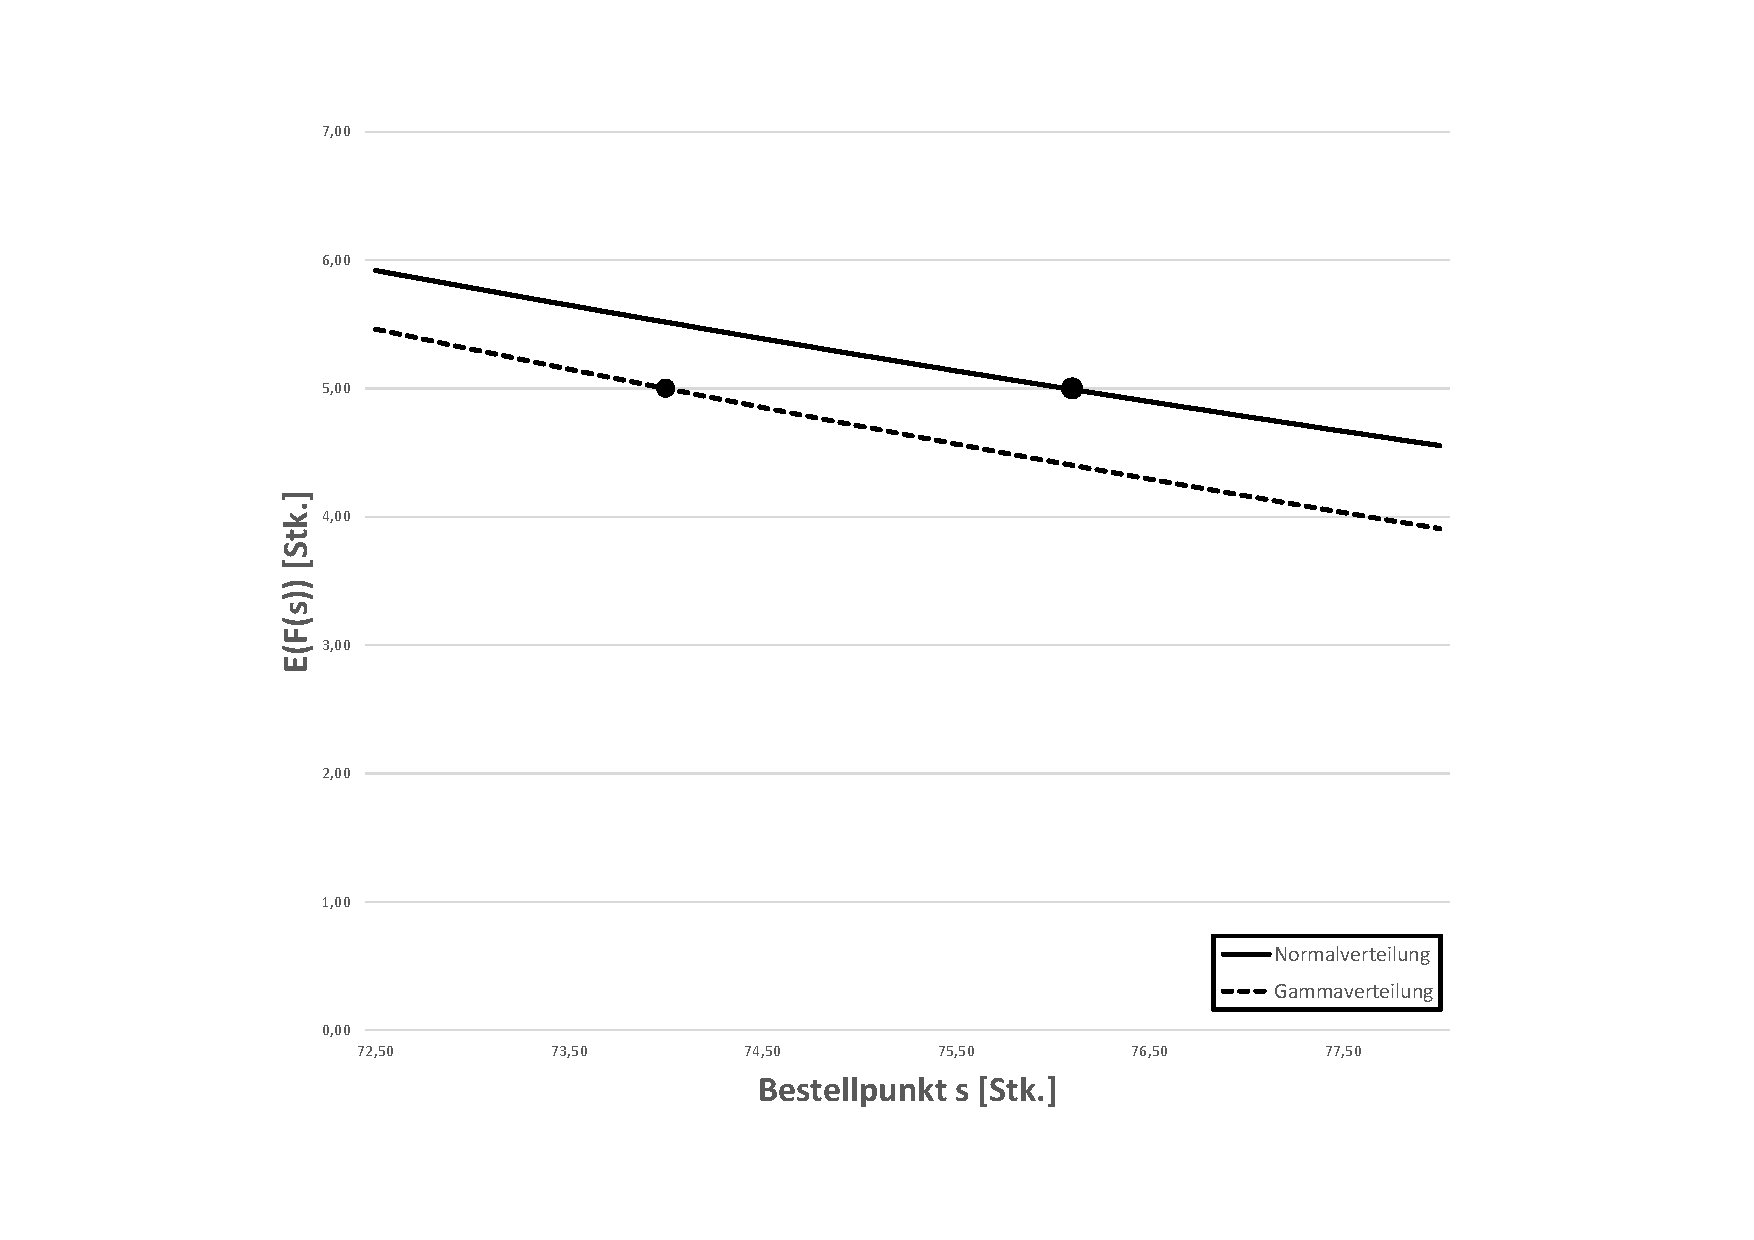
\includegraphics[width=\textwidth,trim=3.7cm 1.5cm 3.3cm 1.5cm, clip=true]{./Bilder/VerteilungsfunktionenVerg.pdf}
	\caption{Vergleich der zu erw. Fehlmengen in Abhängigkeit von s bei Normal- und Gammaverteilung}
	\label{img:vergleich}
\end{figure}